\subsection{Block-Based Adaptive Mesh Refinement (AMR)}
Having discretized the governing equations, the geometry similarly needs to be discretized into unique cells, in a process called meshing. For increase in accuracy, a finer mesh resolution (smaller grid size) will be required. \par

Adaptive Mesh Refinement (AMR) takes its name from the variational increase in localized grid resolution to allow for improved accuracy at without carrying out the same at a ubiquitous scale. Global refinement is often cheaper to perform, whereas localized (Adaptive) is not; however, the computational cost for refining many more cells and storing this information makes it more expensive, in spite of the fact that a well designed approach selection will need to be programmed to perform an adaptive refinement.\par
Block-based AMR groups cells into blocks, making it an optimal configuration for parallel systems, where each processor could have a certain number of Blocks, and protocols such as the Message Passing Interface (MPI) could be used for Block-Block inter-communication. Communication between Blocks occurs via Ghost cells, and in case neighboring blocks have a difference in mesh resolution, then Mutligrid-type restriction and prolongation is used.\par

%parallel here
\begin{figure}
    \vspace{0.2cm}
    \begin{center}
      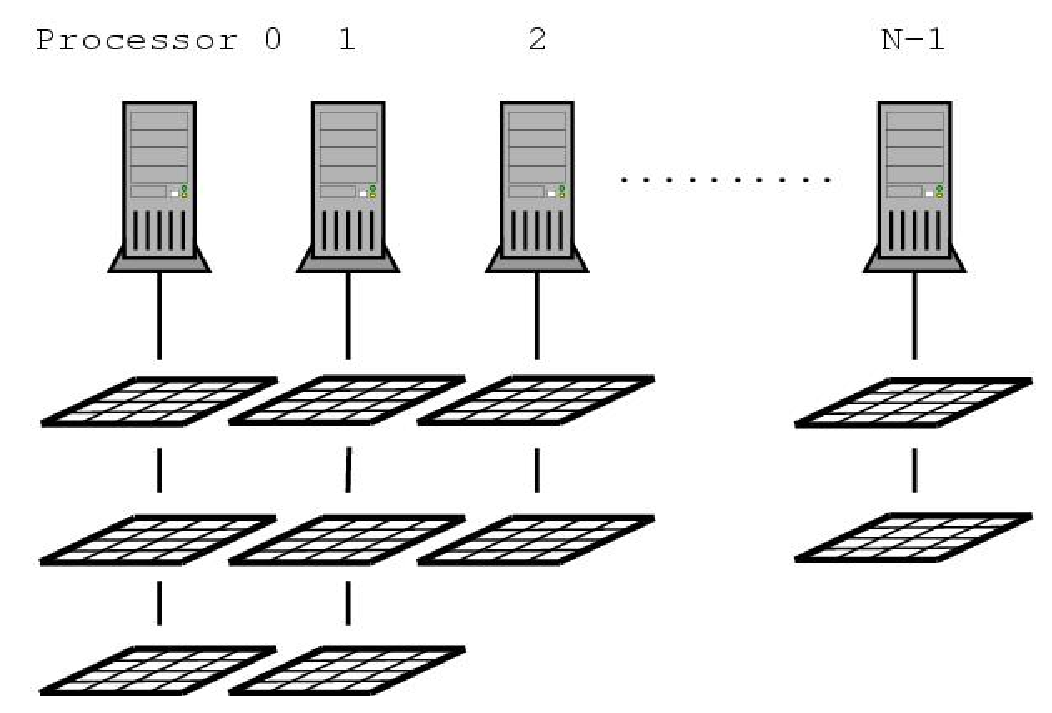
\includegraphics[height=0.35\textwidth]{./figs/parallel-domain-decomp.eps}
    \end{center}
    \caption{Parallel Implementation of Block-based AMR \cite{Northrup:2013}}  
    \vspace{0.2cm}
\end{figure}

Groth \etal ~\cite{Groth:1999} developed some of the initial work with Block-Based AMR for Computational Magnetohydrodynamics, and was extended to enable parallel implementation for a variety of complex flows. Northrup and Groth ~\cite{Northrup:2005b} implemented a fully-implicit, parallel Newton-Krylov method, and applies Schwarz preconditioning to take advantage of the Block structure of the computational grid.
Within Block-based AMR, the cell-connectivity is stored in a tree structure, which will typically be an octree in a 3D domain. Block-Based AMR is more optimized than a refinement performed on a cell-by-cell basis, as the information storage process for the latter is computationally expensive: The tree approach is much simpler, faster and cheaper. Blocks flagged for increased resolution can be refined using two approaches: \par

  
\begin{figure}[t!]
  \centering
   \subfigure[2D Block-Ghost configuration \cite{Northrup:2013}]
   {\label{fig:2D Block}	   
   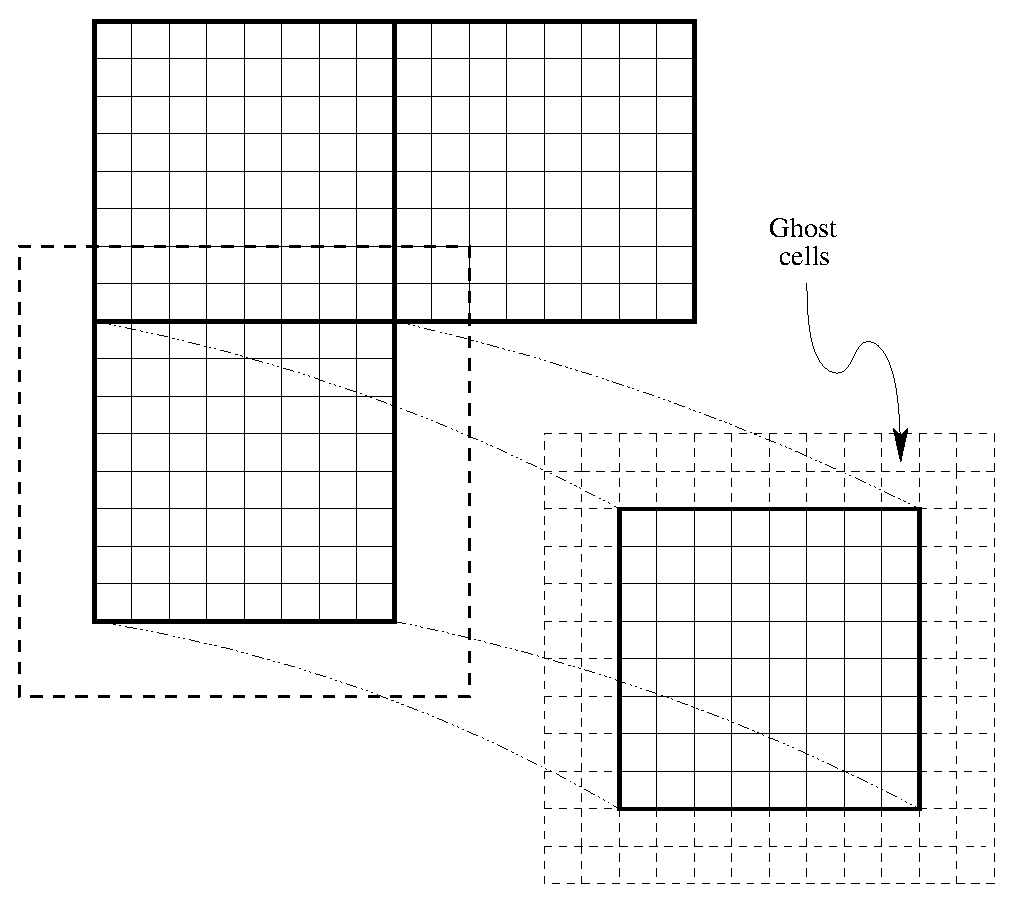
\includegraphics[height=0.35\textwidth, trim=0.2cm 0.2cm 0.2cm .2cm,clip=true]{figs/2dgrid_ghostcells.eps}}%
	\:
	\subfigure[3D Block-Ghost configuration \cite{Northrup:2013}]
   {\label{fig:3D Block}	   
   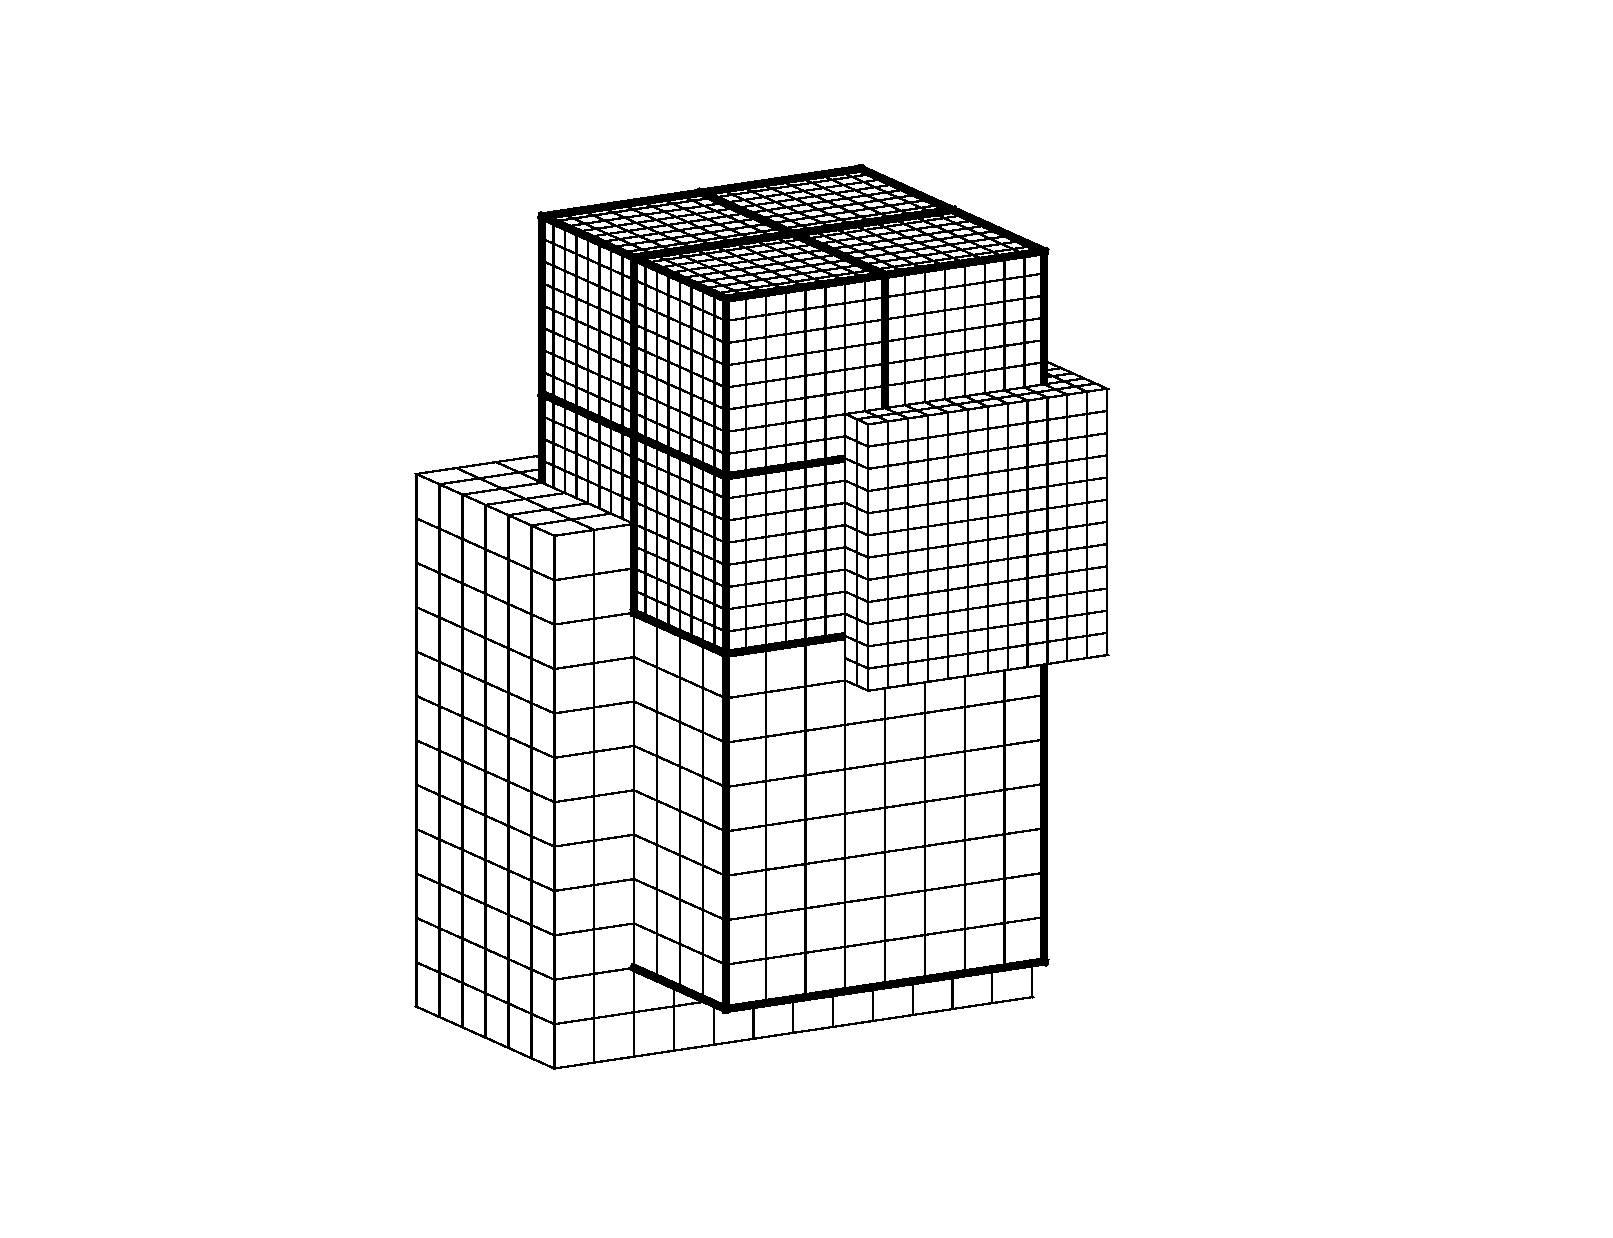
\includegraphics[height=0.35\textwidth, trim=0.2cm 0.2cm 0.2cm .2cm,clip=true]{figs/amr-blocks-ghosts.eps}}%
     \caption{Block structure depicting interior cells and ghost cell configurations}  
\end{figure}  
  

\begin{enumerate}

\item \textbf{Isotropic AMR}:\\
Isotropic AMR  occurs by uniformly splitting the Parent cell into 8 children (in a 3D domain) or into 4 children (in a 2D domain). This considers that the physics is occurring without a preference for a given direction, and usually results in a larger-than-desired cell count.

\begin{figure}
    \vspace{0.2cm}
    \begin{center}
      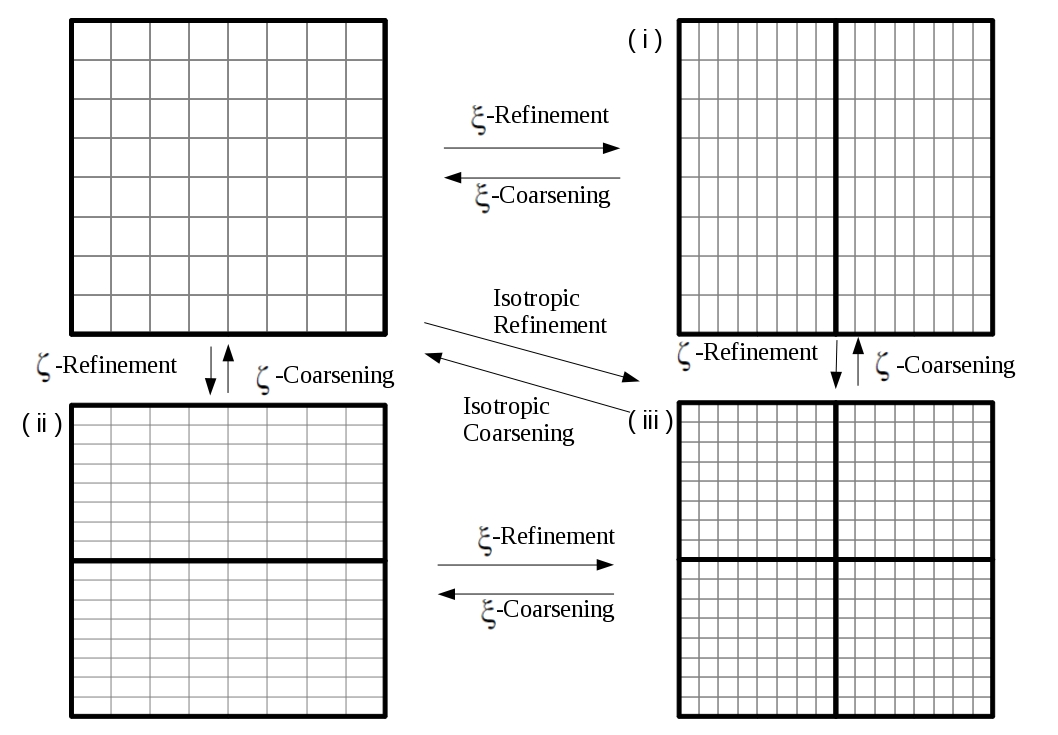
\includegraphics[height=0.35\textwidth]{./figs/BlockDivision.jpg}
    \end{center}
    \caption{Isotropic and Anisotropic AMR \cite{Zhang:2011b}}  
    \vspace{0.2cm}
\end{figure}

\item \textbf{Anisotropic AMR}: \\
For flows having a directional bias, e.g. in the simulation of a jet exiting a nozzle, the dominant direction will be along the axis of symmetry of the nozzle. Therefore, a priori, we can tell that the mesh cells would ideally need to be stretched along this same axis. Whenever we have this kind of bias on the cell geometry, we have anisotropy. Mesh refinement occurs in a slightly different manner, as now we switch to a binary tree system, which stores refinement history and cell connectivity. Two, four, or eight refined blocks can be created, resulting in five distinct possible refinements for a single block to better adapt to evolving flow features. Studies by Zhang ~\cite{Zhang:2011b}, and Zhang and Groth ~\cite{Zhang:2011a} indicate that Anisotropic AMR for given simulations result in lower cell counts, although the refinement procedure is more difficult than that of the Isotropic AMR.\par


Freret and Groth \cite{Freret:2015} have completed a new formulation for a Non-uniform block-based approach that targets the the ghost cells. In this method, a block will copy over the mesh resolution and solution information of its neighboring block to its own ghost cells, and this eliminates the interpolation error within a Uniform block-based scheme that would otherwise have resulted in necessary solution restriction and prolongation (if the mesh discretization levels were different). Further, this saves the computational cost of flux correction cycles, done via message passing between the blocks, as described by Zhang to be a temporary remedy to ghost-cell evaluation.\cite{Zhang:2011a}

\begin{figure}
    \vspace{0.2cm}
    \begin{center}
      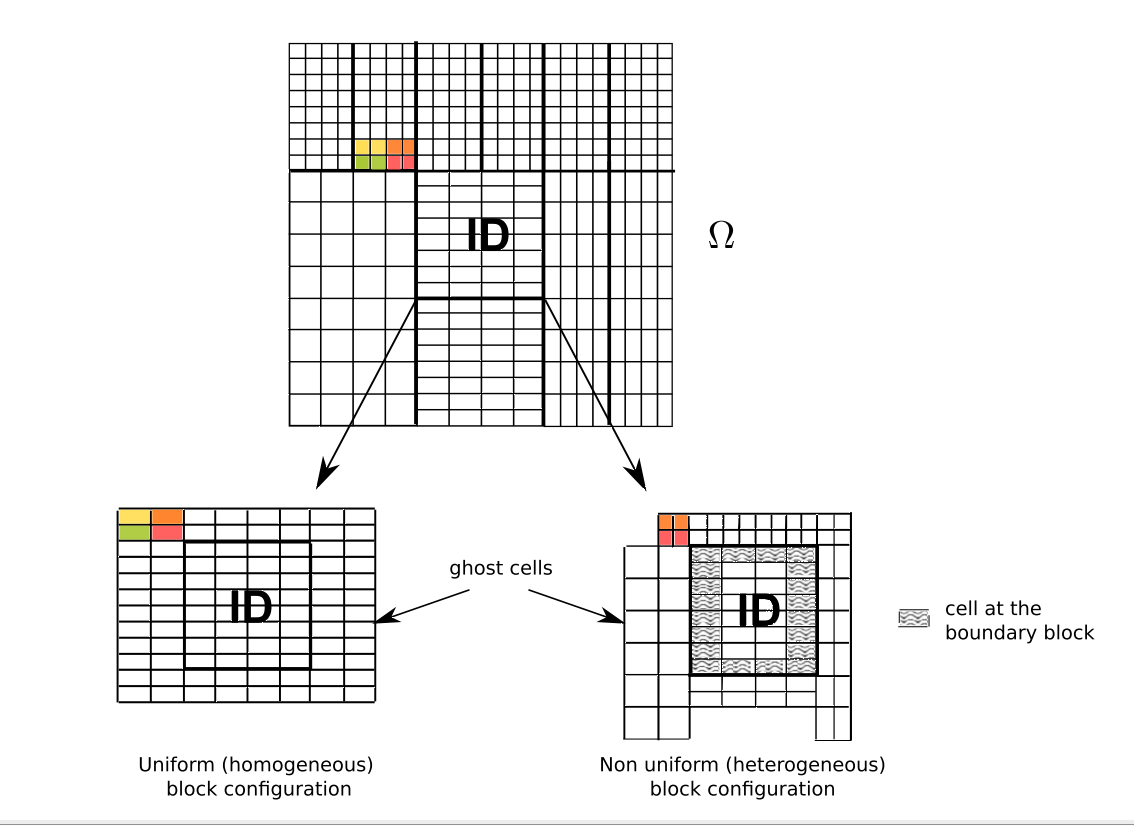
\includegraphics[height=0.35\textwidth]{./figs/Non-UniformBlock.png}
    \end{center}
    \caption{Non-Uniform Ghost Cells on Block \cite{Freret:2015}}  
    \vspace{0.2cm}
\end{figure}

\end{enumerate}
